\section{UNIDAD 1}
    \subsection{Conceptos básicos}

        \begin{center} 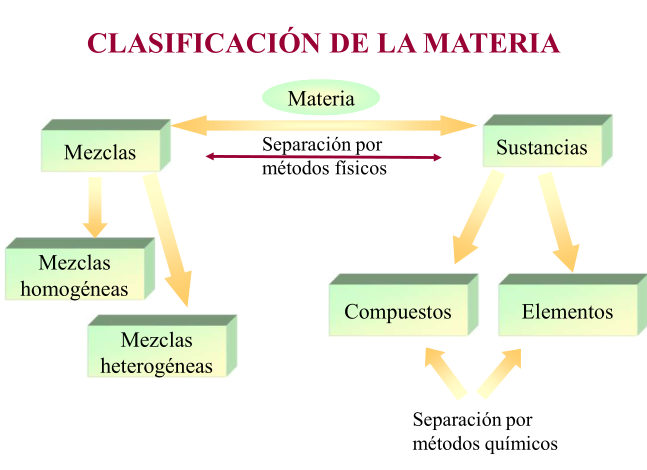
\includegraphics[width=6cm]{./imagenes/clasificacionMateria.png} \end{center}

        \indent La \textcolor{red}{\textit{Química}} es la ciencia que estudia la composición, estructura y propiedades de la materia, conjuntamente con los cambios que ésta sufre. \\
        \indent La \textcolor{red}{\textit{Materia}} es todo lo que ocupa lugar en el espacio y tiene masa. \\
        \indent Una \textcolor{red}{\textit{Sustancia}} es una forma de materia que tiene una composición dada y propiedades específicas que la distinguen de otras. \\
        \indent Una \textcolor{red}{\textit{Mezcla}} es una combinación de dos o más sustancias puras en la que cada una conserva sus propiedades particulares.

        \begin{itemize} 
            \item \textbf{Mezcla homogénea:} composición uniforme de la mezcla.
            \item \textbf{Mezcla heterogénea:} composición no uniforme de la mezcla.
        \end{itemize}   

        Los componentes de una mezcla se pueden separar mediante procesos físicos.

        \indent Un \textcolor{red}{\textit{Elemento}} es una sustancia que no se puede separar en otras más sencillas por medios químicos. \\
        \indent Un \textcolor{red}{compuesto} es una sustancia constituida por átomos de dos o más elementos químicos unidos en proporciones fijas definidas. \\
        Los compuestos sólo se pueden separar en sus elementos puros por medios químicos. \\
       
    \subsection{La materia (estados y propiedades)}
        \indent \textbf{\underline{Los estados de la materia son:}}
            \begin{itemize} 
                \item Sólido
                \item Líquido
                \item Gas
            \end{itemize}

        \indent \textbf{\underline{Cambios:}}
            \begin{itemize}
                \item \textcolor{red}{Físicos:} no altera la estructura o la identidad de una sustancia.
                \item \textcolor{red}{Químicos:} altera la estructura o identidad de la sustancias involucradas.
            \end{itemize} 

        \indent \textbf{\underline{Propiedades:}}
            \begin{itemize}
                \item \textcolor{red}{Extensivas:} son aquellas dependientes de la cantidad de materia considerada.
                \item \textcolor{red}{Intensiva:} propiedad que no depende de la cantidad de materia considerada.
            \end{itemize}
            
    \subsection{Mundo microscópico}
        \indent \textbf{\underline{Átomos, moléculas e iones}}
            \begin{itemize}
                \item \textcolor{red}{Átomo:} partícula más pequeña de un elemento que mantiene su identidad química a través de todos los cambios físicos y químicos. Pueden intervenir en una combinación química. 

                \item \textcolor{red}{Molécula:} unión de dos o más átomos, eléctricamente neutros. Una molécula es la partícula más pequeña de un compuesto o elemento que tiene una existencia estable e independiente.
            \end{itemize}

            \begin{center}
                \underline{Representación del átomo} \\[5pt]
                \ce{^{\scalebox{1.5}{A}}_{\scalebox{1.5}{Z}}\scalebox{1.5}{X}}
            \end{center}

                \begin{itemize}
                    \item \textbf{A:} Número másico; es el número de protones más el número de neutrones.
                    \item \textbf{Z:} Número atómico; es la cantidad de protones en el núcleo.
                    \item \textbf{X:} Es el elemento de la tabla periódica.
                \end{itemize}

            \begin{center} \underline{Moléculas} \end{center}
                \indent Una molécula es un conjunto de dos o más átomos unidos por fuerzas de atracción electrostática.
                \begin{center} 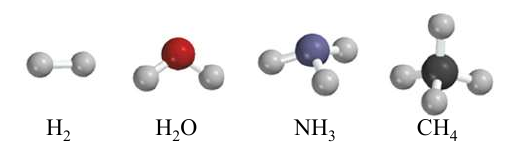
\includegraphics[width=6cm]{./imagenes/moleculas.png} \end{center}
                \begin{itemize}
                    \item Moléculas di-atómicas 

            \begin{center} \underline{Iones} \end{center}
                \indent Un ion es un átomo o grupo de átomos que tiene una carga neta positiva o negativa, distinto a ''eléctricamente neutro''.
                \begin{itemize}
                    \item \textbf{Catión:} es un átomo con carga neta positiva, sucede cuando cede electrones.
                        \begin{center} \ce{^{11}_{11}$Na$} $\rightarrow$ \ce{^{11}_{10}$Na^+$} \end{center}
                    \item \textbf{Anión:} es un átomo que ''acepta'' electrones y su carga es eléctricamente negativa.
                        \begin{center} \ce{^{17}_{17}$Cl$} $\rightarrow$ \ce{^{17}_{18}$Cl^-$} \end{center}
                \end{itemize}
                \indent Los iones pueden clasificarse en función si son uno solo átomo o varios:
                \begin{itemize} 
                    \item Ión mono-atómico: contiene un solo átomo, por ejemplo:
                        \begin{center} ${Na^+},{Cl^-},{Ca^{2+}},{O^{2-}},{Al^{3+}},{N^{3-}}$ \end{center}
                    \item Ión poliatómico: contiene más de un átomo, como por ejemplo:
                        \begin{center} ${OH^-},{CN^-},{{NH_4}^{+}},{{NO_3}^{-}}$ \end{center}
                \end{itemize}
                \saltoPag

            \begin{center} \underline{Isótopos} \end{center}
                \indent Son átomos del mismo elemento pero con un número distinto de neutrones en el núcleo, como por ejemplo:
                \begin{center} \ce{^{235}_{92}$U$} y \ce{^{238}_{92}$U$} \end{center}
                \indent Las propiedades químicas de un elemento están determinadas fundamentalmente por los protones y los electrones, los isótopos tienen similar comportamiento químico, aunque diferente comportamiento físico.

    \subsection{Macro-mundo}
        \begin{center} \underline{Masa atómica} \end{center}
            \indent La \textcolor{magenta}{Masa atómica} es la masa de un átomo en unidades de masa atómica (uma).
            \begin{center} \textit{1 átomo \ce{^{12}_{}$C$} ''pesa'' 12 uma} \end{center}
            \indent Suele ser conveniente expresar un porcentaje de ''uma'' de un elemento con respecto al \ce{^{12}_{}$C$}. Por ejemplo, el \ce{^{1}_{}$H$} tiene un peso de 1,008 uma, el 8,4\% de la masa del \ce{^{12}_{}$C$}.
            \begin{itemize} \item \textbf{Masa atómica promedio} \end{itemize}
            \indent El litio, como todos los elementos de la naturaleza, se encuentra en forma de isótopos. Algunos de ellos son: \begin{center} 7,42\% \ce{^{6}_{}$Li$} (6,015 uma) \\ 92,58\% \ce{^{7}_{}$Li$} (7,016 uma) \end{center}
            \begin{center} $M_P = \frac{\sum{(porcentaje)(masa atomica)}}{100}$ \end{center}
            \begin{center} $M_P = \frac{(7,42)(6,015) + (92,58)(7,016)}{100} = 6,941 uma$ \end{center}

        \begin{center} \underline{Moles} \end{center}
            \indent Se entiende como mol a la cantidad de sustancia que contiene tantos átomos como hay en exactamente 12 gramos de \ce{^{12}_{}$C$} y es igual al número de Avogadro ($N_A$).
            \begin{center} $1 mol = N_A = 6,0221367 \times 10^{23}$ \end{center}

        \begin{center} \underline{Masa molar} \end{center}
            \indent La masa molar es la masa molecular expresada en gramos, y como la suma de las masas atómicas de los elementos de un compuesto. Para cualquier elemento, la masa atómica (uma) = masa molar (gramos).
            \begin{center} 1 mol de átomos de $\ce{^{12}_{}C} = N_A = 12g$ \end{center}
            \begin{itemize}
                \item $\mathcal{M}$ = masa molar en $\frac{g}{mol}$ 
                \item $N_A$ = Número de Avogadro (partículas/mol)
            \end{itemize}

            \indent Ejemplo: el $SO_2$
            \begin{center}
                \begin{tabular}{| c | c | c |}
                    \hline
                    Elementos & Masa molar & Cant. \\
                    \hline \hline
                            S & 32,07g     & 1mol \\
                    \hline
                            O & 16g        & 2mol \\
                    \hline
                \end{tabular}
            \end{center}
            \begin{center}
                \begin{tabular}{|c|}
                    \hline
                    $SO_2$ = \textcolor{red}{64,07g} \\
                    \hline
                \end{tabular}
            \end{center}
            \indent Entonces, en 1 $mol$ de $SO_2$ hay 64,07g. A su vez, en el número de Avogadro hay esa masa.
            \begin{center} 1 $mol$ de $SO_2$ = 64,07g = 6,022 $\times$ $10^{23}$ \end{center}
